\chapter{Impulse Response}\label{impulseTestAppendix} 
\textbf{Name: Group 630}\\
\textbf{Date: 11/03 - 2016}

\subsubsection{Purpose}
Observe the impulse response of the Cubli hanging upside down.

Data is used to compare the response of measured response and the simulation given by the theoretical nonlinear model.

\subsubsection{Setup}
The Cubli is put upside down under a table with 2 clamps placed at each side of the bottom plate of the Cubli setup.
The wheel is being held in a fixed position with a strip tied to it and the frame. The probe chosen is a 1:1 and is connected to the potentiometer with probe to yellow cable and ground clamp to brown cable. The power supply has to be connected, and turned on, to the Cubli in order to get readouts from the potentiometer.
\begin{figure}[H] 
	\centering 
	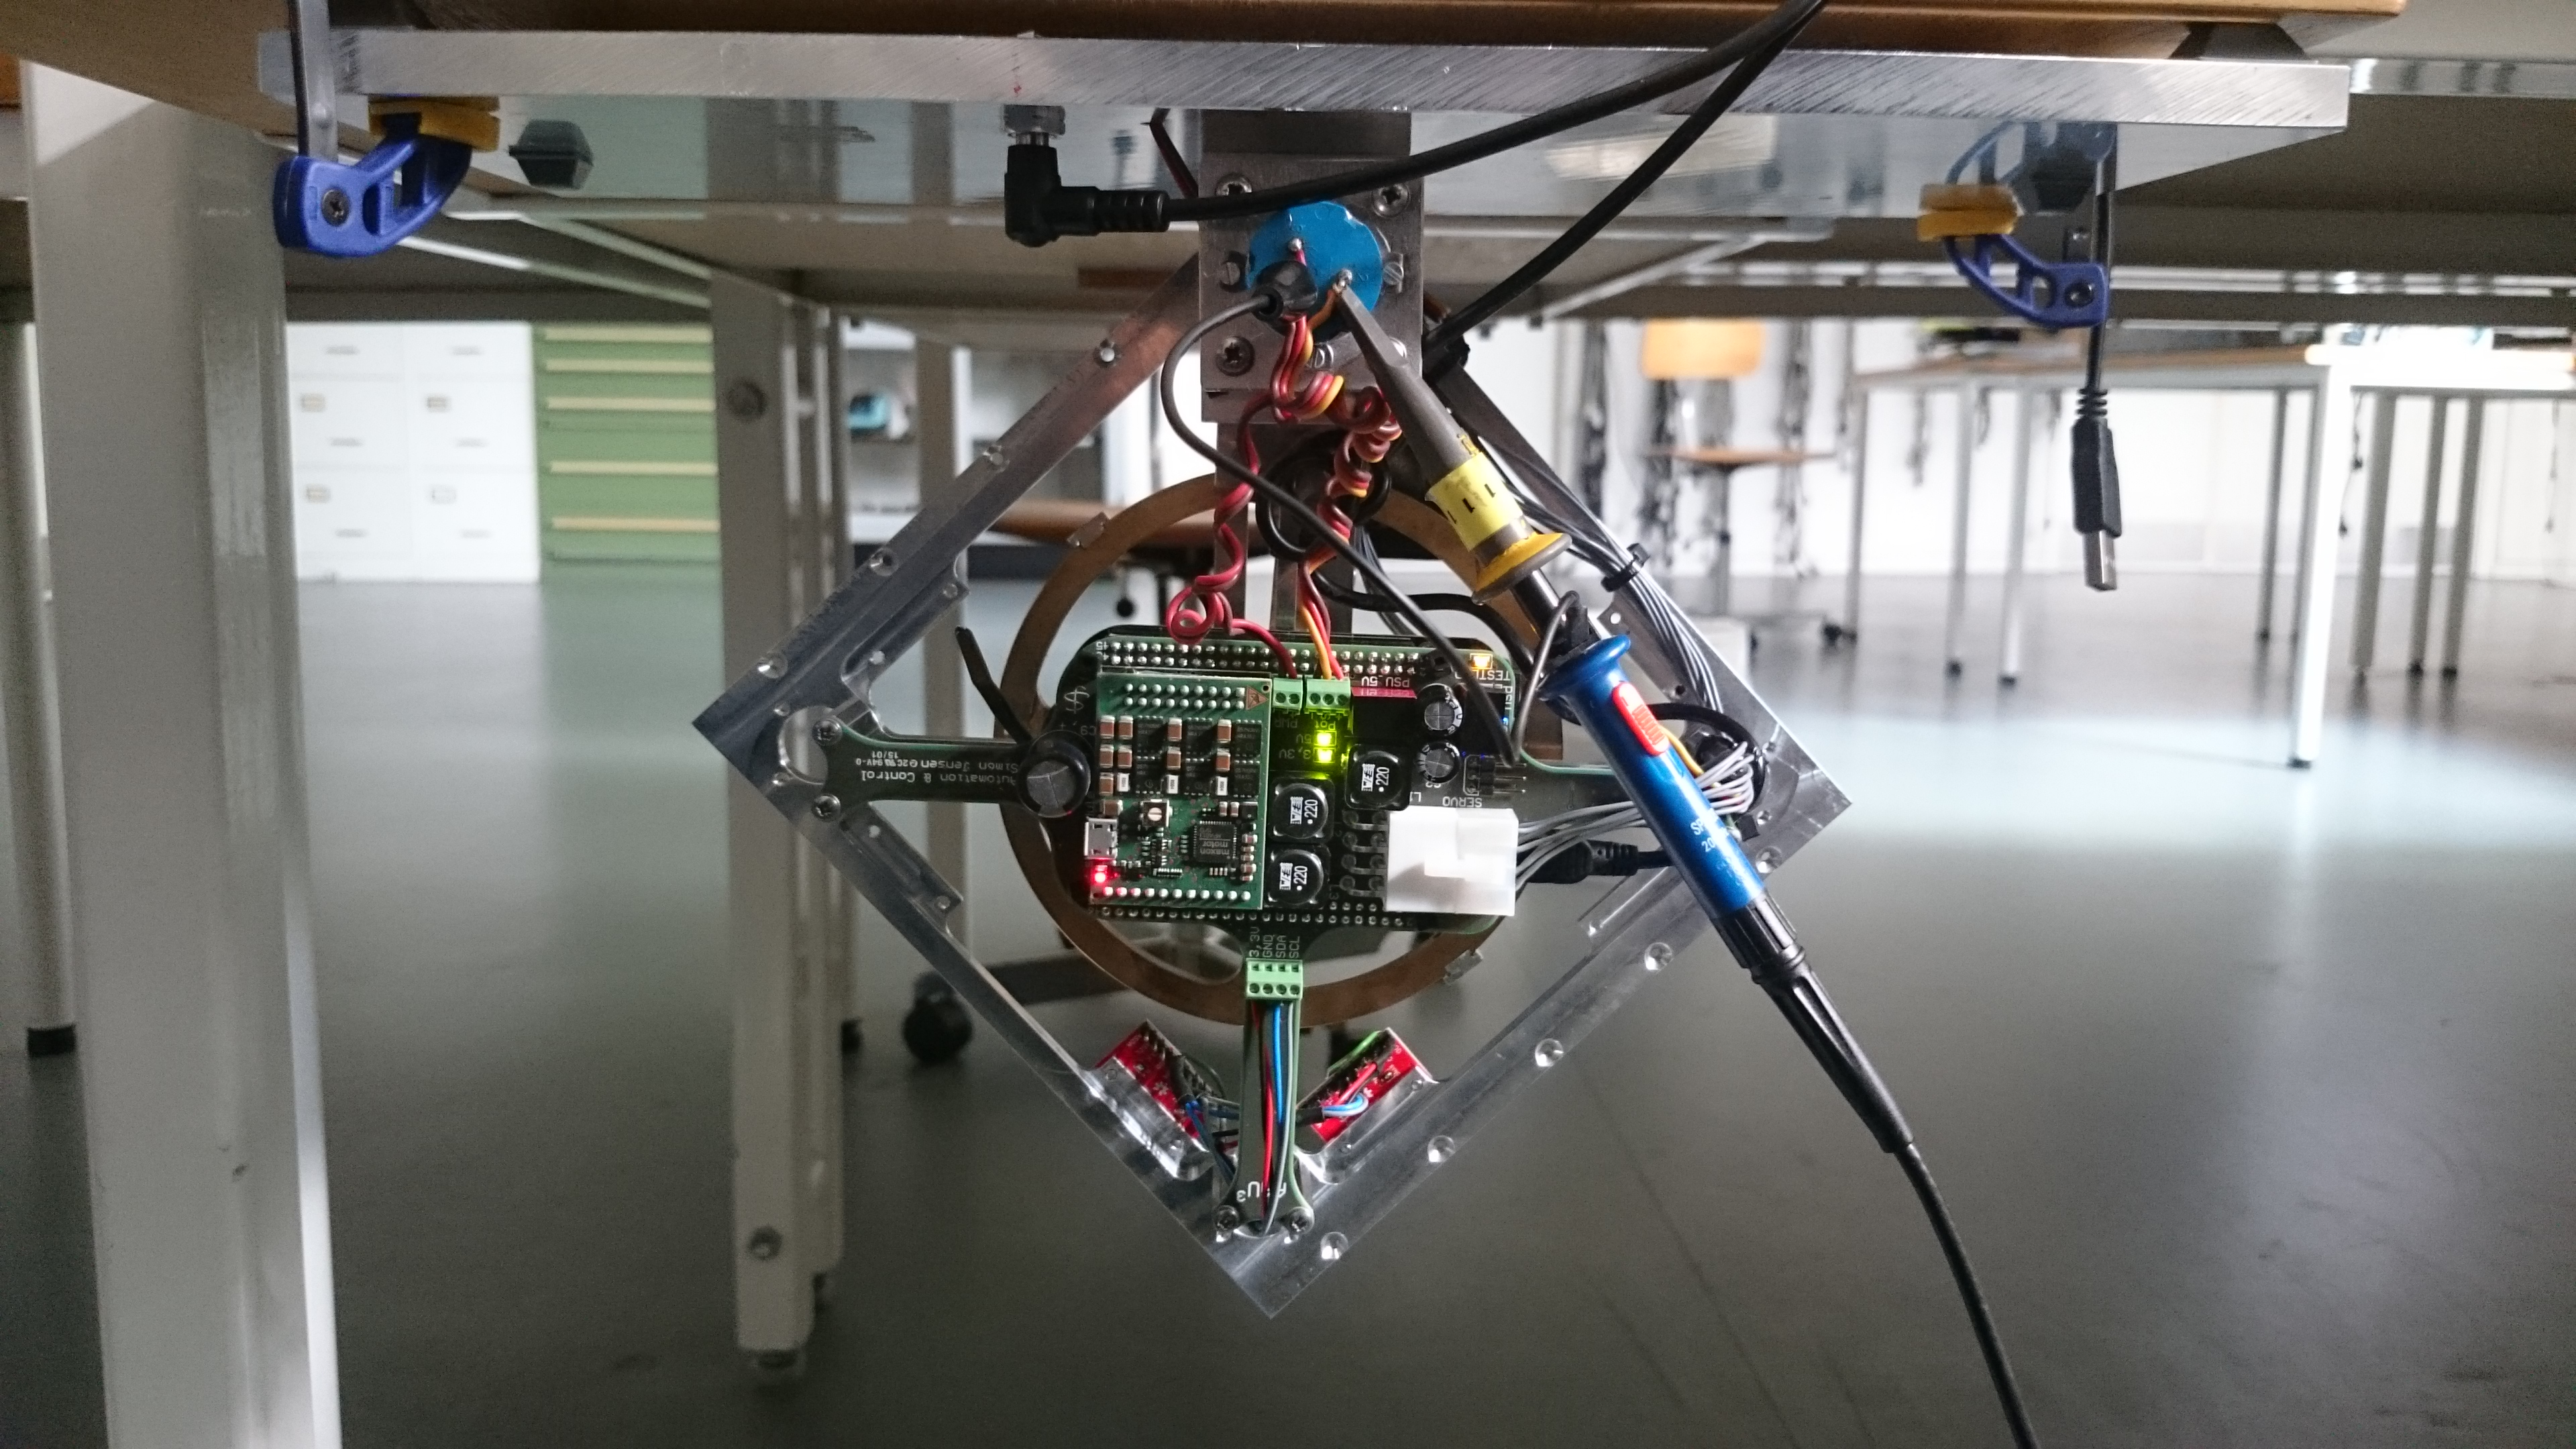
\includegraphics[scale=0.08]{figures/impulseResponseSetup}
	\caption{The Cubli setup hanging upside down beneath a table during the impulse response test}
	\label{impulseResponseTestPicture}
\end{figure} 

\subsubsection{List of Equipment}
\begin{table}[H]
	\begin{tabular}{|l|l|p{4cm}|}
		\hline%------------------------------------------------------------------------------------
		\textbf{Instrument}                        &  \textbf{AAU-no.}  &  \textbf{Type}       \\
		\hline%------------------------------------------------------------------------------------
		Cubli setup                              &               &  		  					\\
		\hline%------------------------------------------------------------------------------------
		Oscilloscope                              &  61604             &  Agilent 54621A		  \\
		\hline%------------------------------------------------------------------------------------
		Dedicated Power Supply of Cubli \small{(24 V - 3 A)} &               &  XP Power, AEB70US24 \\
		\hline%------------------------------------------------------------------------------------
		Probe 1:1                &  TBD            		&          TBD\fxnote{find the probe used}  \\
		\hline%------------------------------------------------------------------------------------
		2x Clamp                &  			            &          							   \\
		\hline%------------------------------------------------------------------------------------
	\end{tabular}
\end{table}

\subsubsection{Procedure}
\begin{enumerate}
	%\item Turn on the power supply
	\item Place the setup upside-down and place the frame touching the base %, \si{135^0} with respect to the vertical position
	\item Let the Cubli fall and swing until it has come to rest
	\item Use the oscilloscope to measure the changes in the potentiometer
	\item Collect all the data and plot it in Matlab
%	\item Compare with the simulation 
	
\end{enumerate}

\subsubsection{Results}
%\begin{figure}[H] 
%	\centering 
%	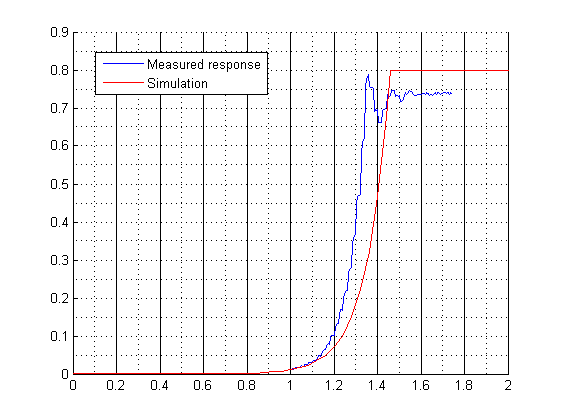
\includegraphics[scale=0.9]{figures/comparisonRealModel}
%	\caption{Comparison between the real behavior and the simulation of the linearized model}
%	\label{comparisonRealModel}
%\end{figure} 

\subsubsection{Note}
During this experiment it was observed that if the frame was released from the left position (The right upper side on \figref{impulseResponseTestPicture} since the Cubli is upside down), the frame would hit the rubber pad on the other side. This behavior was not observed when releasing the Cubli from the right position (left upper corner).

\subsubsection{Conclusions}